%----------------------------------------------------------------------------------------
%	PACKAGES AND OTHER DOCUMENT CONFIGURATIONS
%----------------------------------------------------------------------------------------

\documentclass[a0paper,portrait]{baposter}

\usepackage[font=small,labelfont=bf]{caption} % Required for specifying captions to tables and figures
\usepackage{booktabs} % Horizontal rules in tables
\usepackage{relsize} % Used for making text smaller in some places

\usepackage{amsmath,amsfonts,amssymb,amsthm} % Math packages
\usepackage{eqparbox}

\usepackage{textcomp}

\usepackage[brazil]{babel}
\usepackage[utf8]{inputenc}

\usepackage{wrapfig}

\graphicspath{{figures/}} % Directory in which figures are stored

 \definecolor{bordercol}{RGB}{45, 235, 118} % Border color of content boxes
 \definecolor{headercol1}{RGB}{5, 184, 255} % Background color for the header in the content boxes (left side)
 \definecolor{headercol2}{RGB}{26, 167, 85} % Background color for the header in the content boxes (right side)
 \definecolor{headerfontcol}{RGB}{0, 0, 0} % Text color for the header text in the content boxes
 \definecolor{boxcolor}{RGB}{255, 255, 255} % Background color for the content in the content boxes


\begin{document}

\background{% Set the background to an image (background.pdf)
\begin{tikzpicture}[remember picture,overlay]
\draw (current page.north west)+(-2em,2em) node[anchor=north west]
{
\includegraphics[height=1.1\textheight]{background}};
\end{tikzpicture}
}

\begin{poster}
{grid=false,
borderColor=bordercol, % Border color of content boxes
headerColorOne=headercol1, % Background color for the header in the content boxes (left side)
headerColorTwo=headercol2, % Background color for the header in the content boxes (right side)
headerFontColor=headerfontcol, % Text color for the header text in the content boxes
boxColorOne=boxcolor, % Background color for the content in the content boxes
headershape=roundedright, % Specify the rounded corner in the content box headers
headerfont=\Large\sf\bf, % Font modifiers for the text in the content box headers
textborder=rectangle,
background=user,
headerborder=open, % Change to closed for a line under the content box headers
boxshade=plain
}
{\begin{tabular}{c}
        
\includegraphics[height=1cm]{UNIVAP-SF.png}\\
\end{tabular}
}
%
%----------------------------------------------------------------------------------------
%	TITLE AND AUTHOR NAME
%----------------------------------------------------------------------------------------
%
{\bf  \LARGE {DECIMETRIC RADIO EMISSION ANALYSIS OF CHROMOSPHERIC EVAPORATION IN A X1.0 FLARE ON MARCH 29, 2014} \\ % Poster title
\vspace{0.2cm}
\footnotesize \underline{André Rossi Korol}, Francisco Carlos Rocha Fernandes\\  % Author names
\footnotesize \it UNIVAP --- Universidade do Vale do Paraíba\\ % Institution names
\footnotesize \it \textcolor{blue}{\underline{anrobits@yahoo.com.br}}\/}
%Author email addresses

{\begin{tabular}{c}
        
\includegraphics[height=1cm]{ipd2-sf.png}
\end{tabular}
}

%----------------------------------------------------------------------------------------
%	RESUMO
%----------------------------------------------------------------------------------------
\headerbox{Abstract}{name=abstract,span=1,column=0,row=0}
{One instance of the chromospheric evaporation phenomenon, associated with a X1.0
    solar flare, was identified by line profile data (Li et al. 2015) recorded by
    the Interface Region Imaging Spectrograph (IRIS;\@ De Pontieu et al. 2014) and
    the EUV Imaging Spectrometer (EIS;\@ Culhane et al. 2007). The present work analyses
    the metric radio emission counterpart of that flare. However, since a slow drift
    rate towards lower frequencies (Aschwanden \& Benz 1995) was not found in the
    resulting spectra, we elaborate on why the chromospheric evaporation could be 
    visualized with line profile data but not with metric radio emission data.

\textit{Keywords: solar flare, solar radio emission,}\newline
\textit{chromospheric evaporation, spectrometer,}\newline
\textit{data analysis, data visualization.}
%Cabe aos autores providenciarem o pôster em material adequado (lona, pvc, glosspaper ou similar) com corda para ser afixado.
}

%---------------------------------------------------------------------------------------
%   INTRODUÇÃO
%---------------------------------------------------------------------------------------

\headerbox{Introduction}{name=introduction,span=1,column=0,below=abstract}
{\begin{center}
        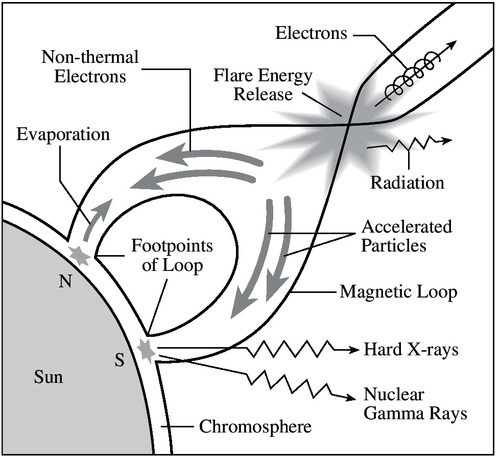
\includegraphics[width=0.8\textwidth]{figures/solar-flare-model.jpg}

        Figura 1. Solar Flare Model\\
        Source: K.R. Lang, Tufts University, 2010.
    \end{center}
}

%----------------------------------------------------------------------------------------
%	OBJETIVOS
%----------------------------------------------------------------------------------------



\headerbox{Objectives}{name=objectives,span=1,column=0,below=introduction}
{The main goal was to visualize the presence or absence of chromospheric evaporation in spectra
    generated from the analysis of metric radio emission data. This general objective was accomplished
    by first achieving the following specific objectives:
    \begin{itemize}
        \item Identification of the time when the event occured
        \item Data selection based on the time found in the previous goal
        \item 
    \end{itemize}

}

%----------------------------------------------------------------------------------------
%	METODOLOGIA
%----------------------------------------------------------------------------------------
\headerbox{Methodology}{name=methodology,span=1,column=1,row=0}
{Pode-se incluir tabelas utilizando o ambiente \texttt{table} ou conforme apresentado abaixo.

Enquanto equações são organizadas utilizando o ambiente \texttt{equation}, como segue:
}

%----------------------------------------------------------------------------------------
%	RESULTADO
%----------------------------------------------------------------------------------------
\headerbox{Results and Discussions}{name=results,span=1,column=1,below=methodology}
{Pode-se incluir figuras utilizando o ambiente \texttt{includegraphics} ou conforme apresentado abaixo.

\begin{center}
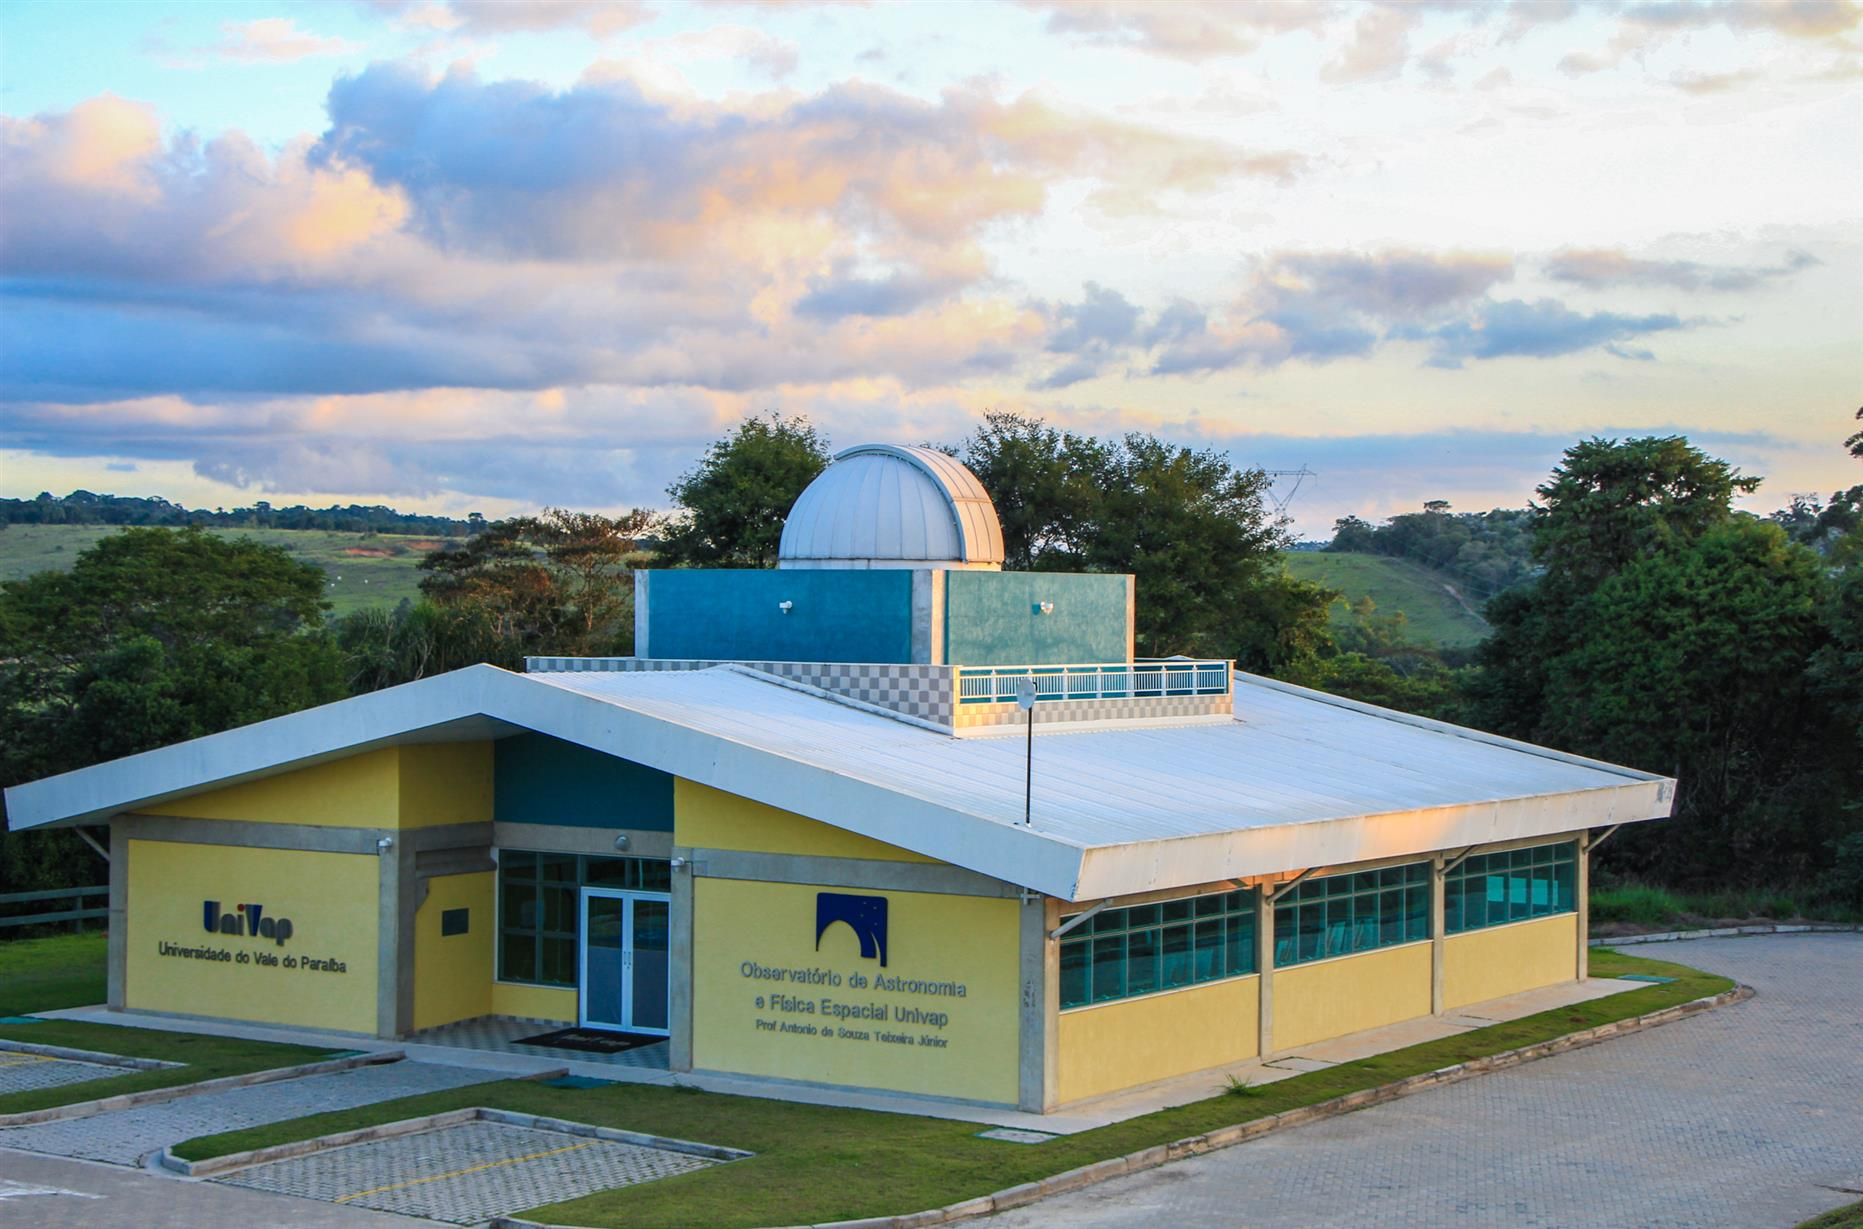
\includegraphics[width=0.8\textwidth]{figures/observatorio.jpg}\\
Figura 1. Posicionar legenda abaixo da imagem, espaçamento simples.\\
Fonte: do autor.
\end{center}

}

%----------------------------------------------------------------------------------------
%	DISCUSSÃO
%----------------------------------------------------------------------------------------
\headerbox{Conclusions}{name=conclusions,column=2,row=0} % To reduce this block to 1 column width, remove 'span=2'
{Sugestões para fazer uma conclusão:
\begin{itemize}
    \item Fazer um breve resumo do trabalho.
    \item Referir qual foi a grande conclusão do trabalho.
    \item Referir se concretizaram ou não todos os objetivos ou se não foi possível concretizar algum deles e explicar o porquê.
    \item Referir a importância que o trabalho tem para sua pesquisa.
\end{itemize}


}

%----------------------------------------------------------------------------------------
%	AGRADECIMENTOS
%----------------------------------------------------------------------------------------
\headerbox{Acknowledgements}{name=acknowledgements,column=2,below=conclusions,span=1}
{A.R. Korol would like to thank PIBIC-Univap for his CNPq scientific initiation grant.\\
    F.C.R. Fernandes thanks FAPESP (Proc. 2017/02806--3) and CNPq (Proc. 311376/2015--0).\\
    Both the authors are thankful to the Institute for Data Science FHNW Brugg/Windisch, Switzerland,
    for the data that is freely available on the e-Callisto network.
}

%----------------------------------------------------------------------------------------
%	REFERENCIAS
%----------------------------------------------------------------------------------------
\headerbox{References}{name=references,column=2,below=acknowledgements,span=1}
{[1] Li, Y., et al. 2015, ApJ, 811, 7

[2] De Pontieu, B., Title, A. M., Lemen, J. R., et al. 2014, SoPh, 289, 2733

[3] Culhane, J. L., Harra, L. K., James, A. M., et al. 2007, SoPh, 243, 19

[4] Aschwanden, M. J., Benz, A. O. 1995, ApJ, 438, 997–1012

}

%----------------------------------------------------------------------------------------
%	REALIZAÇÃO
%----------------------------------------------------------------------------------------

\headerbox{Realization}{name=event,column=0,below=references, above=bottom,span=3}
{\begin{center}
    
\includegraphics[width=0.7\textwidth]{rodape_simfast.png}
\end{center}
}


\end{poster}

\end{document}
